Organize this section according to the rules defined in the project description. 
\subsection{External Interface Requirements}
\subsubsection{User Interfaces}
\subsubsection{Hardware Interfaces}
\subsubsection{Software Interfaces}
\subsubsection{Communication Interfaces}
\subsection{Scenarios}
\begin{enumerate}
\item[•]{\Large Scenario 1} \\
The company StatisticsDispenser is interested into weekly providing public statistics about people living in London. For this reason the company, which is already registered to Data4Help, need to send a group monitoring request. After logging into the Data4Help website, StatisticsDispenser open the group request section. The website loads a new page where the company can filter groups through some attributes regarding his members like the age, the gender, the city and many more. For the specific purpose StatisticsDispenser chooses only to filter people who live in London and people who's age is between 20 and 60. Then, due to the fact that the company need future data, StatisticsDispenser subscribes to the group. From now on every time new data is available the system sends a notification to StatisticsDispencer. 
\item[•]{\Large Scenario 2}
L'utente si registra in una partner application
\item[•]{\Large Scenario 3}
L'utente collega l'account in una partner application
\item[•]{\Large Scenario 4}
Ambulanza viene mandata (ricordati che il diagramma è sbagliato)
\item[•]{\Large Scenario 5}
Promote a run
\item[•]{\Large Scenario 6}
spectate a run

\end{enumerate}

\subsection{Functional Requirements}
\begin{enumerate}
\item[•]{\Large Data4Help}
	\begin{enumerate}
	\item [G.1] \textbf{Collect users' position and health status.}
		\begin{enumerate}
		\item [D.1] Users' information are collected from partner applications or from the other two TrackMe applications installed on users' devices.
		\item [D.2] All the partner applications require to submit user credentials.
		\item [D.3] The identification (fiscal code, social security number) and the secondary data (attributes) given by the individual during the registration are correct.
		\item [R.1] Retrieve user credentials inserted into partner application as group attributes.
		\item [R.2] Allow users already registered in Data4Help world to sign in with his account without provide user credentials again.
		\item [R.3] Allow individuals to agree with privacy policy (first part). Registered users, now, can be tracked in group mode request through installed application.  
		\item [R.4] Allow individuals to specify, during registration, if they are also interested to be tracked in single mode request (second part) through installed application.  .
		\item [D.4] Devices used to monitor individuals always work and report 			the correct values.	
    	\item [D.5] Partner application always report correct values to Data4Help.
    	\item [R.5] The system has to correctly receive data from partner applications installed on users' device.
    	\end{enumerate}	
    	
    \item [G.2] \textbf{Provide to Third Parties, the users' position and heath status.}
    	\begin{enumerate} 
    	\item [R.6] Allow third parties registration to Data4Help service, where they have to specify all their credentials.
    	\end{enumerate}	
		
		\begin{enumerate} 
		\item [G.2.1] \textbf{Provide data on-demand to non-subscribed third parties.}
		\begin{enumerate} 
		\item [R.7] For each user registered ,the system has to automatically retrieve and store data from partner applications with a resolution of 10 minutes; independently from the requests reached.	
		\item [R.8] The system has to collect inside his database all the useful information that match the request.
		\item [R.9] The system has to send to applicant all the data already collected.
    	\end{enumerate}	
    	
    	\item [G.2.2] \textbf{Provide data in real-time to subscribed third parties.}
		\begin{enumerate}
		\item [D.8] Live acquisition lasts 24 hours to reduce waste of resources.
    	\item [R.10] Allow third parties subscription to interested group in order to receive live data.
    	\item [R.11] When a real time request is performed the system has to collect and store specific users' data with a resolution of 2 minutes.
    	\item [R.12] Provide to subscribed third parties data as soon as they are available by the system.
    	\end{enumerate}
    	\end{enumerate}
    
	\item [G.3] \textbf{Allow third parties two different ways to get users' data.}
		\begin{enumerate}     
    	\item [G.3.1] \textbf{Allow third parties to get data of a single person.}
		\begin{enumerate}
		\item [D.6] In order to perform an individual request, third parties has to know the user's fiscal code or security number.
		\item [D.7] Security number and fiscal code are not information given to third parties by Data4Help.
    	\item [R.13] Allow third parties to insert fiscal code of user that want to track.
    	\item [R.14] Deny third parties to receive information about users in  single mode, that have not accepted second part of privacy policy.
    	\item [R.15] Collect all the useful information retrieved by Data4Help that are produced by the interested users 
    	\item [R.16] Send all the collected information to request applicant.
    	\end{enumerate}
    
    	\item [G.3.2] \textbf{Allow third parties to get data of a group of people.}
		\begin{enumerate}
    	\item [R.17] Allow third parties to insert attributes in which they are interested to restrict their field of search.
    	\item [R.18] Deny third parties to receive information if the provided information can hurt users' privacy, for this purpose group request under 1000 users involved are rejected.
    	\item [R.15] Collect all the useful information retrieved by Data4Help that are produced by the interested users 
    	\item [R.16] Send all the collected information to request applicant.
    	\end{enumerate}
    	\end{enumerate}
    	
    \item [G.4] \textbf{Provide data in an anonymous way, to protect users' privacy.}
		\begin{enumerate}
    	\item [R.14] Deny third parties to receive information about users in  single mode, that have not accepted second part of privacy policy.
    	\item [R.18] Deny third parties to receive information if the provided information can hurt users' privacy, for this purpose group request under 1000 users involved are rejected.
    	\end{enumerate}	
			
	\end{enumerate}
	
	
\item[•]{\Large AutomatedSOS}
	
	\begin{enumerate}
	\item [G.5] \textbf{Retrieve user's position and health status.}
		\begin{enumerate}
		\item [R.19] Allow users to be tracked from AutomatedSOS filling up the registration and agreeing to both parts of privacy policy.
		\item [D.4] Devices used to monitor individuals always report correct values.
		\item [D.9] The user always dresses a smartwatch on which AutomatedSOS is installed.    
		\item [R.20] The application has to interact with Smartwatch/Smartphone APIs in order to retrieve location and health status.
		\item [R.21] The application is able to send to Data4Help service all the informations already retrieved in live acquisition.
		\end{enumerate}
		
	\item [G.6] \textbf{Allow health-interested third parties the access to data detected by AutomatedSOS.}
		\begin{enumerate}
		\item [R.22] Allow non-profit organizations to register into AutoatedSOS portal and becoming health third parties.
		\item [R.23] Allow health third parties to receive informations about all the users registered to AutomatedSOS through Live Acquisition performed by Data4Help.
		\end{enumerate}
	
	\item [G.7] \textbf{Monitor user's health parameters.}
		\begin{enumerate}
		\item [R.20] The application has to interact with Smartwatch/Smartphone APIs in order to retrieve location and health status.
		\item [R.24] The application has to retrieve users' health status every 2 seconds in order to guarantee reaction time of 5 seconds.
		\end{enumerate}
		
	\item [G.8] \textbf{Send an ambulance to users' location whenever certain parameters are below the threshold.}
		\begin{enumerate}
		\item [R.25] The application has to control health status with data retrieved in local to realize immediately if certain parameters are critical.
		\item [R.26] The application has to call an ambulance, if parameters are critical.
		\item [D.10] The ambulance system is always up and ready to receive messages from AutomatedSOS.
		\item [R.27] Supply to hospital user's location and all the useful information to provide efficient first aid.
		\item [D.11] The ambulance successfully reach the location of the individual.
		\end{enumerate}
		
  	\end{enumerate}
  	
  	
\item[•]{\Large Track4Run}
	
	\begin{enumerate}
	\item [G.5] \textbf{Retrieve user's position and health status.}
		\begin{enumerate}
		\item [R.28] Allow users to be tracked from Track4Run filling up the registration and agreeing to both parts of privacy policy.
		\item [D.4] Devices used to monitor individuals always report correct values.
		\item [R.20] The application has to interact with Smartwatch/Smartphone APIs in order to retrieve location and health status.
		\item [R.21] The application is able to send to Data4Help service all the informations already retrieved in live acquisition.
		\item [R.28] The application is able to send to Data4Help service updated daata with a resolution of 5 seconds.
		\end{enumerate}
		
	\item [G.9] \textbf{Allow promoters to manage a run.}
		\begin{enumerate}
		\item [R.29] Allow users to create a run providing all the general information about the competition.
		\item [R.30] Allow users to specify if the race is public or private.
		\item [D.4] Devices used to monitor individuals always report correct values.
		\item [D.13] During a run athletes always dress a smartwatch on which Track4Run is installed.
			
		\item [G.9.1] \textbf{Allow promoters to define a path for the run.}
			\begin{enumerate}
			\item [R.31] Allow promoters to define a path for the race by selecting the routes inside a map.
			\item [D.14] The path defined by the organizer actually exist.
			\end{enumerate}
			
		\item [G.9.2] \textbf{Allow promoters to invite athletes to the run.}
			\begin{enumerate}
			\item [R.32] Allow promoters to invite athlete to be runner of their private race.
			\item [R.33] Allow promoters to specify maximum number of athletes that can take part to their public race.
			\end{enumerate}
	\end{enumerate}
	
	\item [G.10] \textbf{Allow athletes to enroll on a specific run.}
		\begin{enumerate}
		\item [R.34] Allow users to see all the public races and private races in which he is invited.
		\item [R.35] Allow user to select a race and add him to the athletes involved.
		\item [D.16] If an athlete enroll to a run then he also participates to the run.
		\end{enumerate}
	
	\item [G.11] \textbf{Allow spectators to watch in real time the position of every athletes in a specific run.}
		\begin{enumerate}
		\item [D.17] All athletes have their tracking devices with them and the application enabled for the entire duration of the run.	
		\item [R.36] Allow user to select a race to be viewed.
		\item [R.37] The application must be able to request to Data4Help the positions of all the other athletes involved.
		\item [R.38] The application must be able to receive and display the positions of all the other athletes involved.
		\item [D.18] Athletes never go out of the defined path.
		\end{enumerate}
	\end{enumerate}

\end{enumerate}

\subsubsection{Use Case Diagram}
\begin{enumerate}
\begin{minipage}{\textwidth}
\FloatBarrier
\item[•]{\Large Data4Help}

\begin{center}
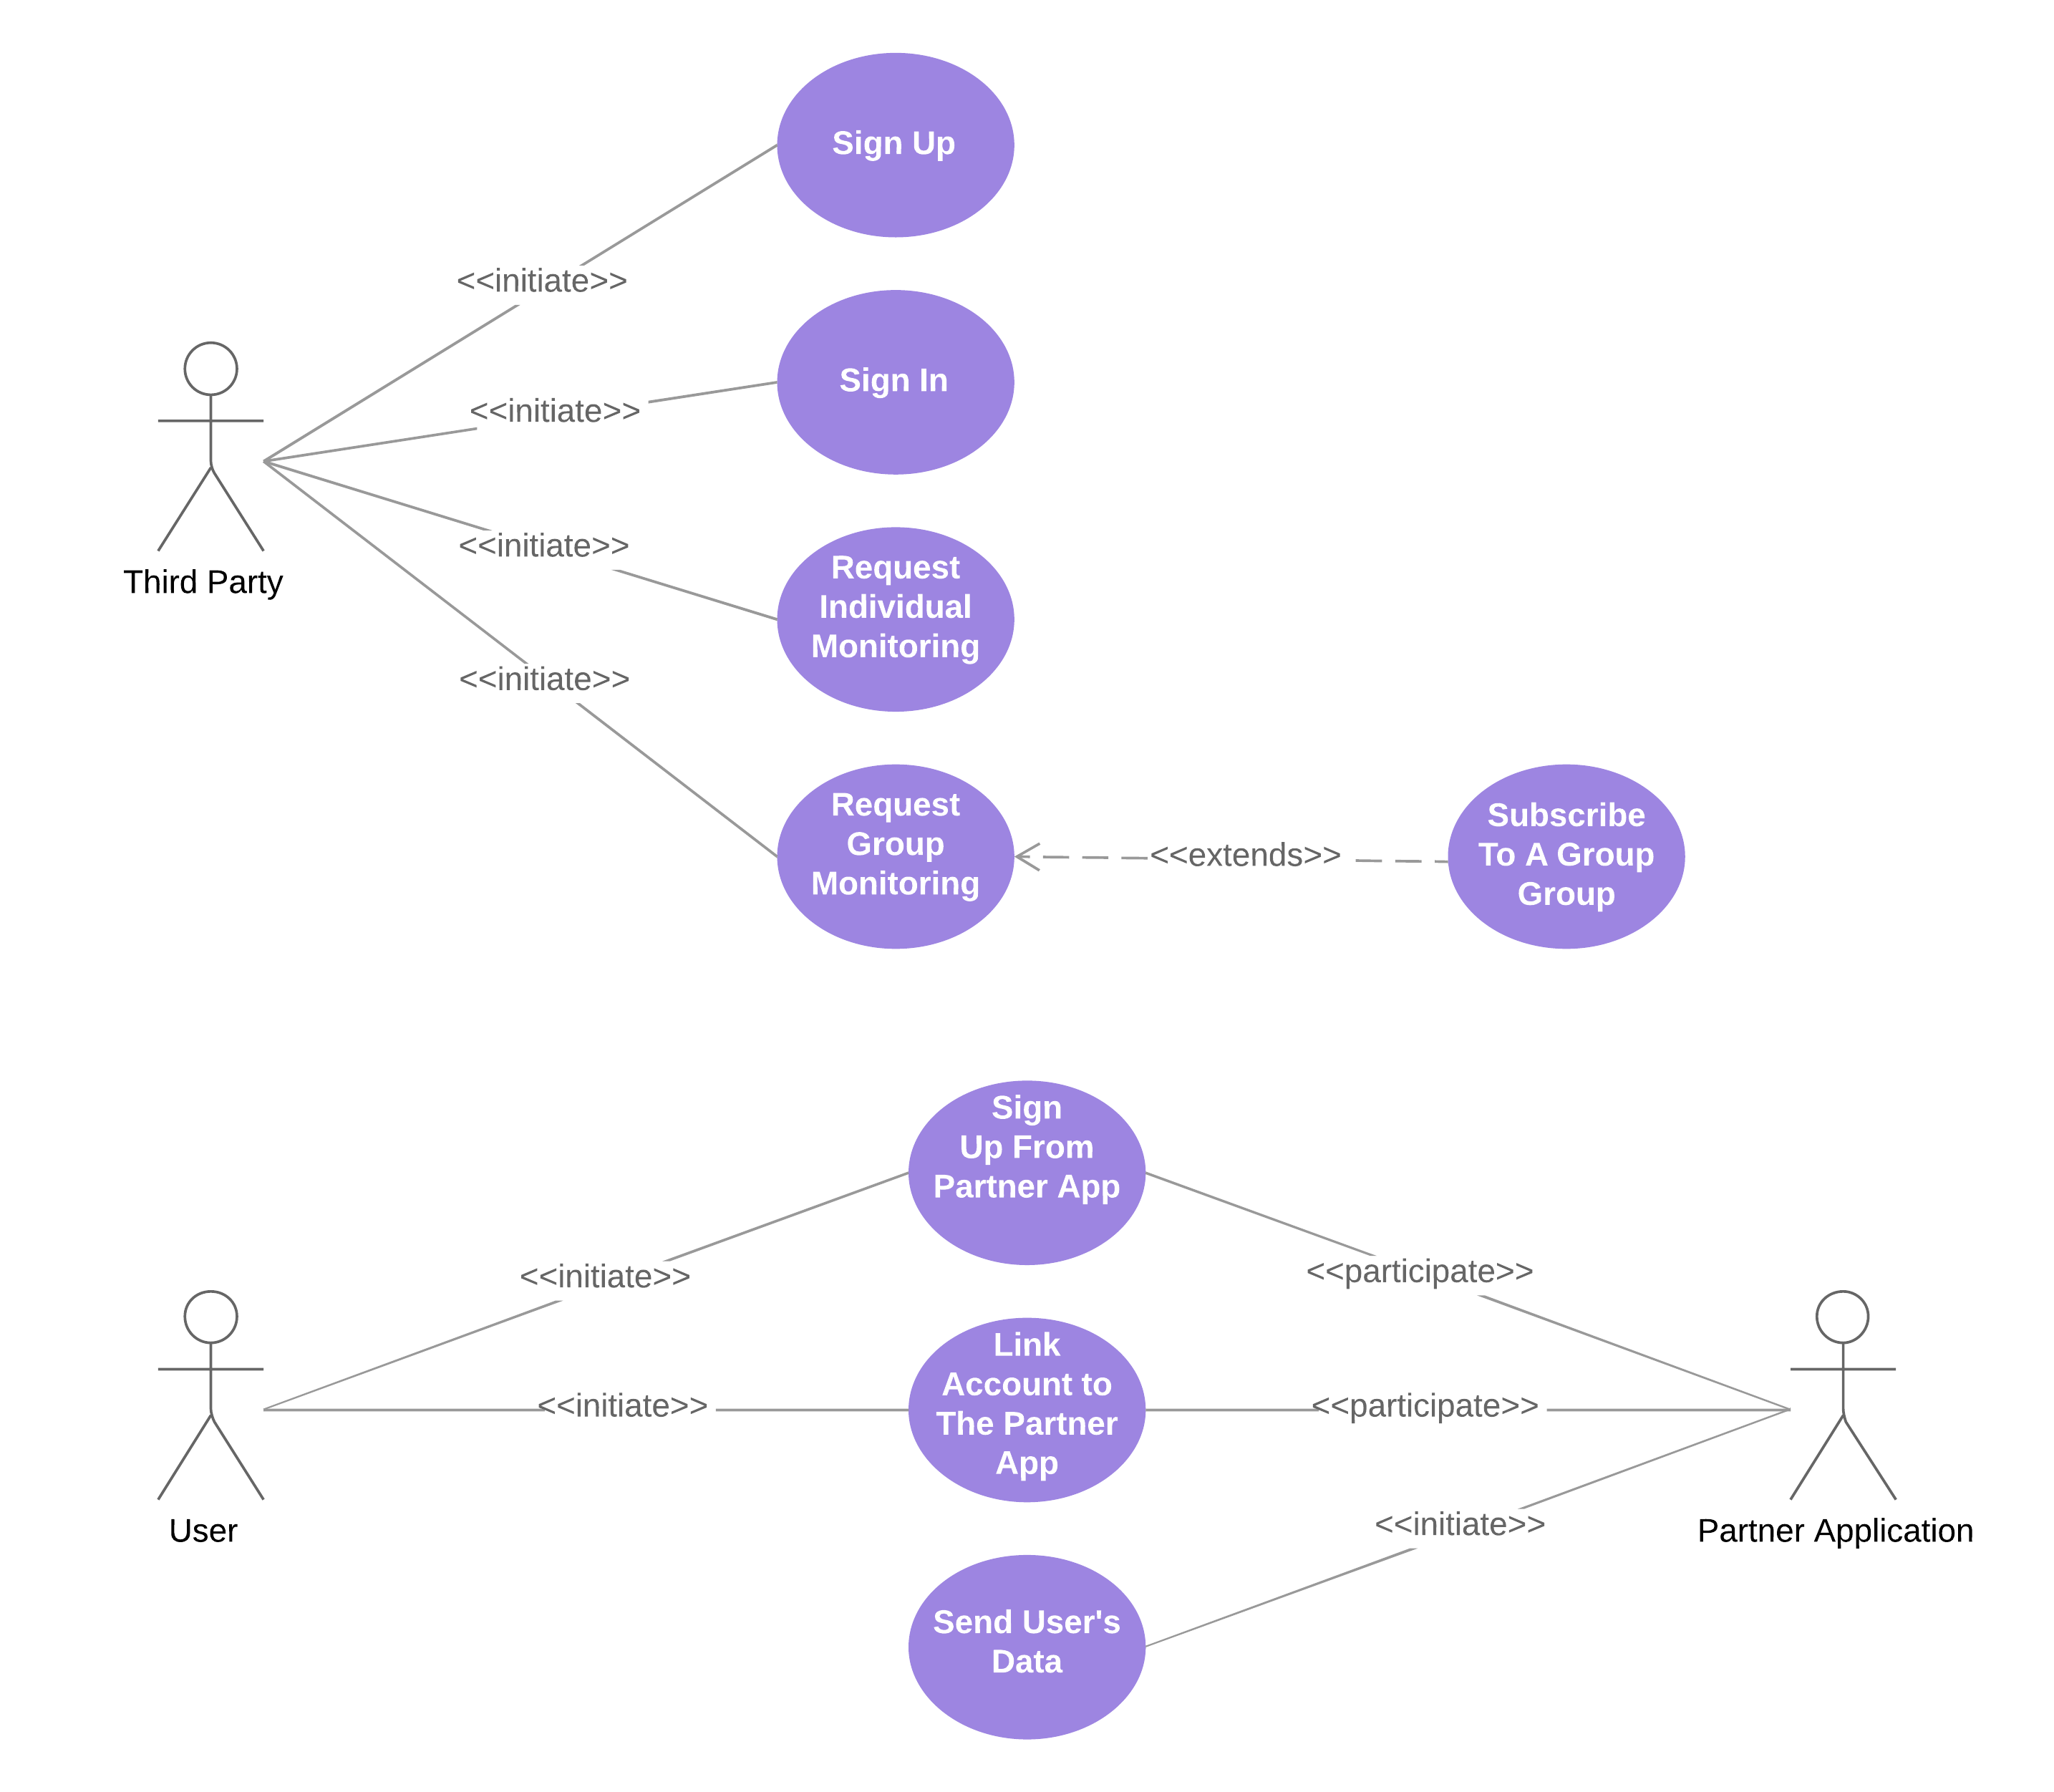
\includegraphics[scale=0.65]{Images/Data4HelpUseCaseDiagram.png}
\end{center}
\FloatBarrier
\end{minipage}


\begin{minipage}{\textwidth}
\item[•]{\Large AutomatedSOS}
\FloatBarrier
\begin{center}
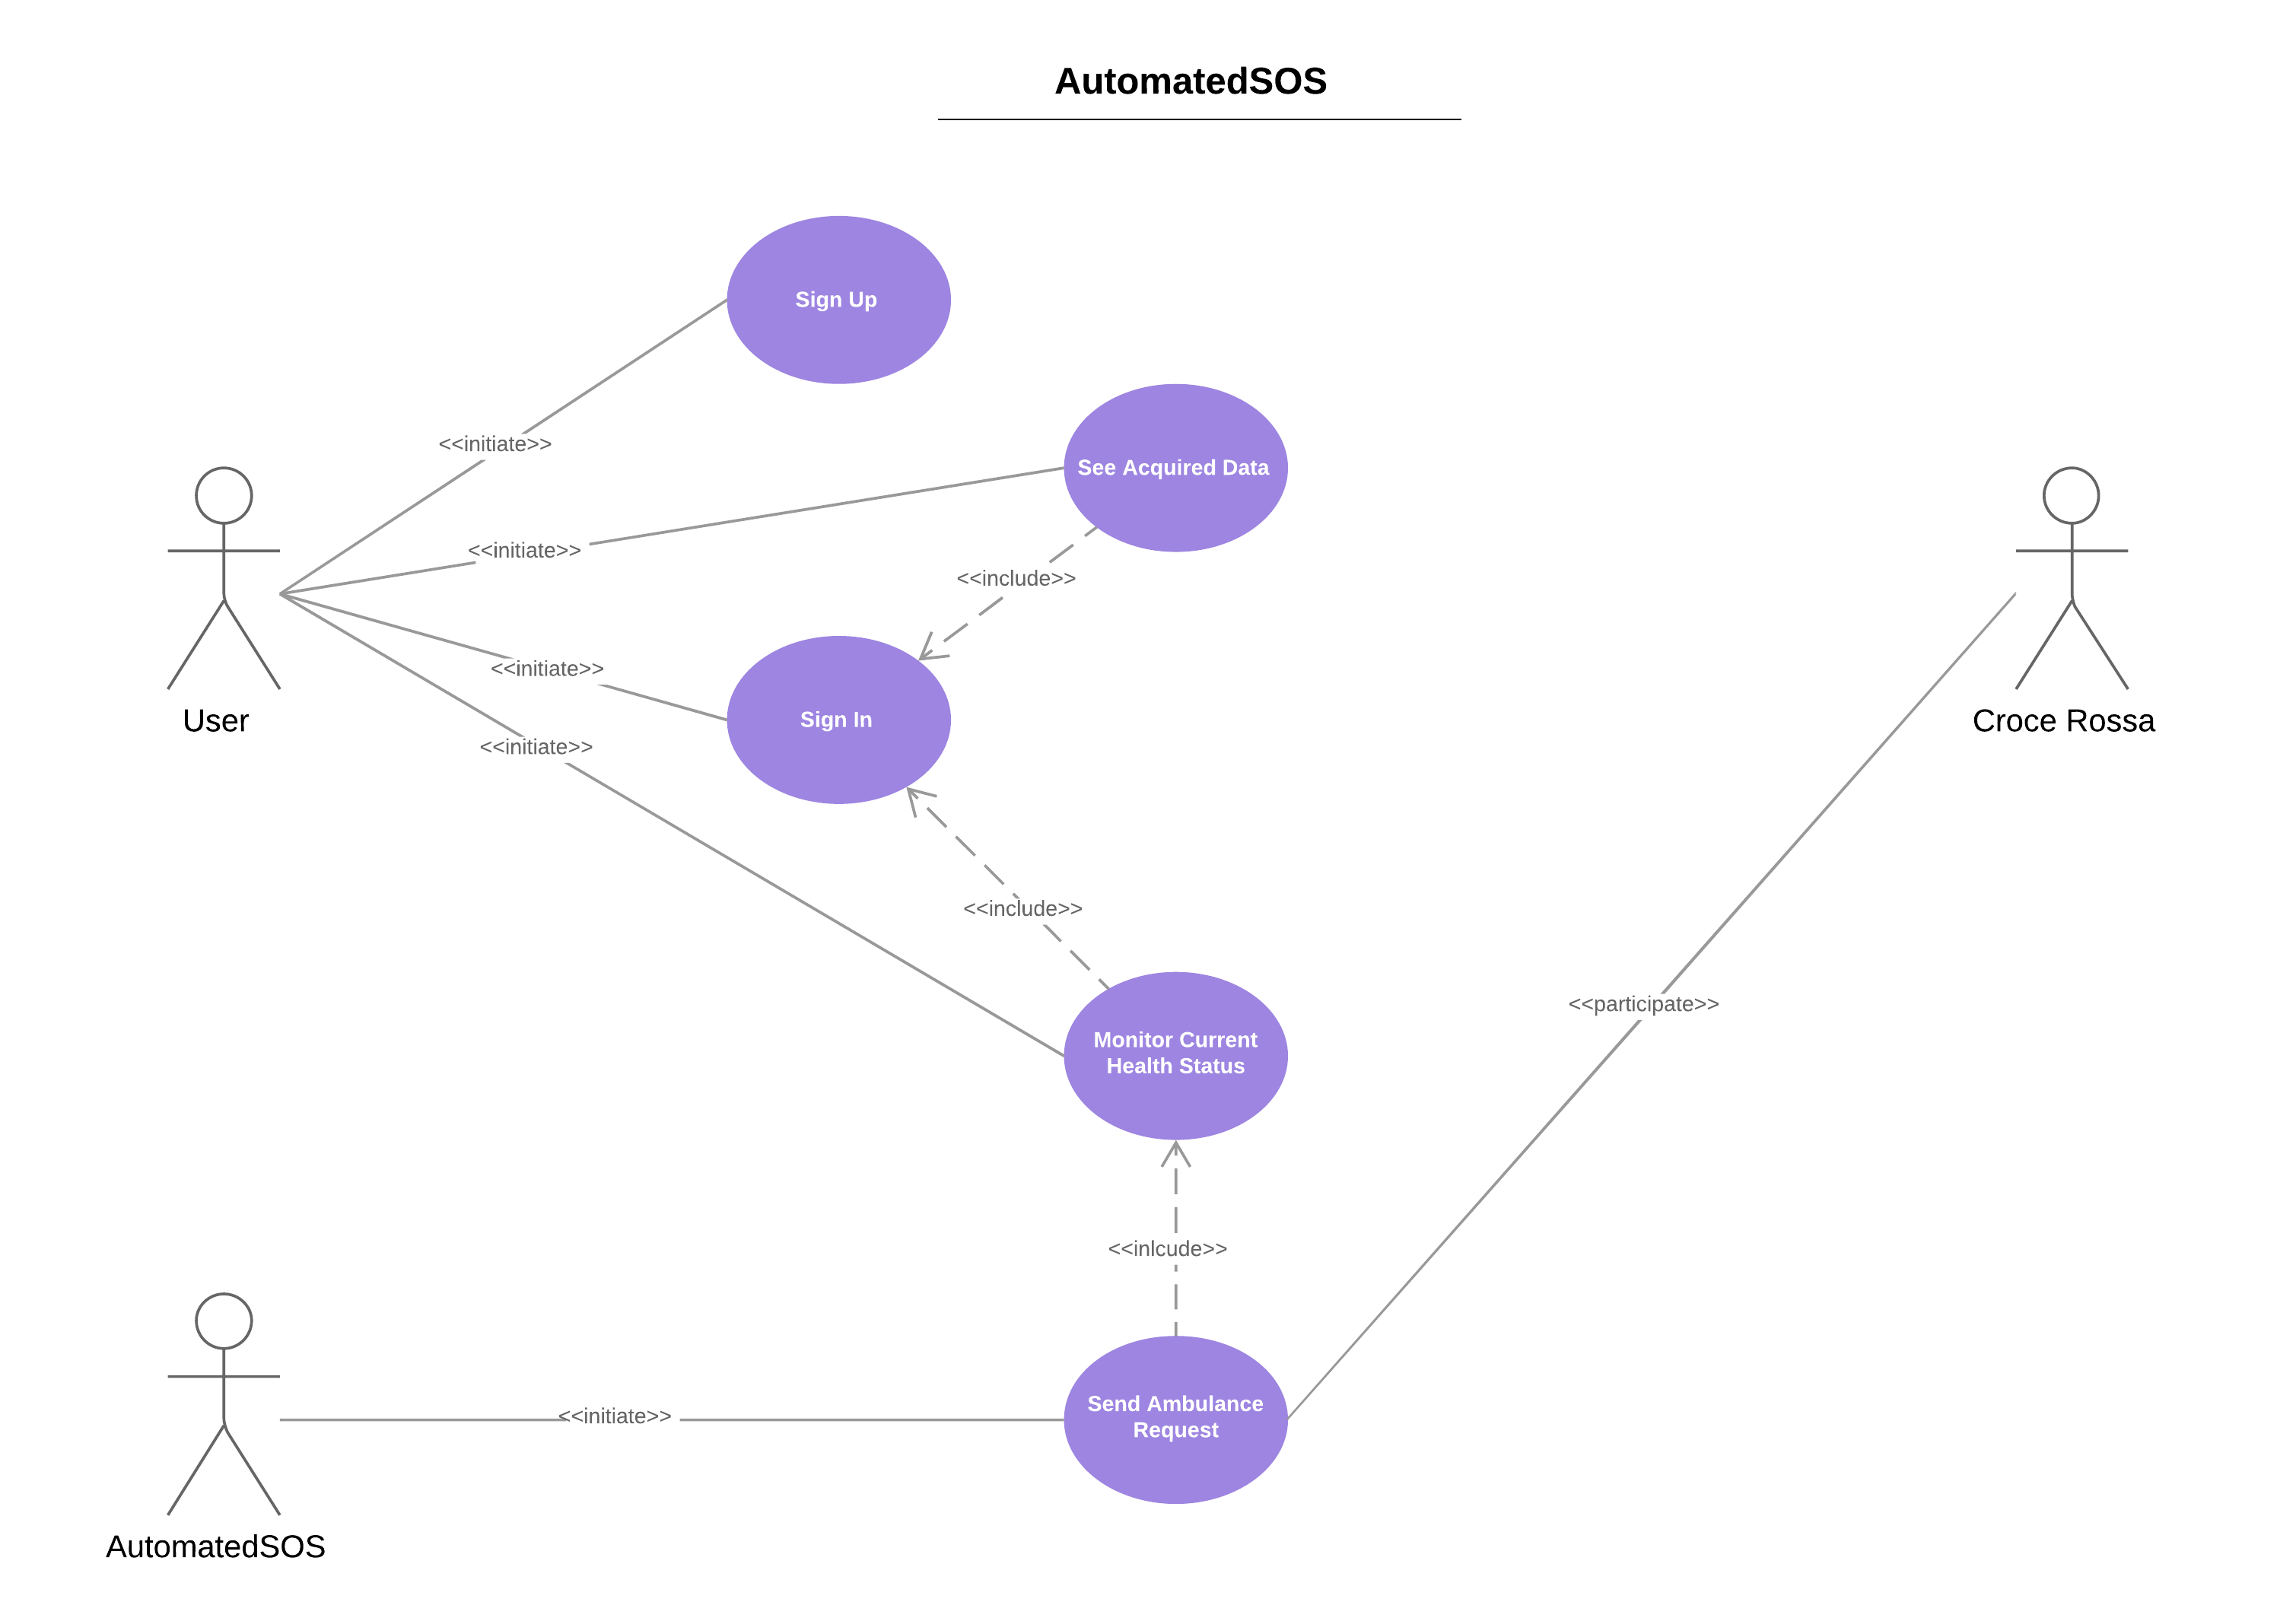
\includegraphics[scale=0.65]{Images/AutomatedSOSCaseDiagram.png}
\end{center}
\FloatBarrier
\end{minipage}

\begin{minipage}{\textwidth}
\item[•]{\Large Track4Run}
\FloatBarrier
\begin{center}
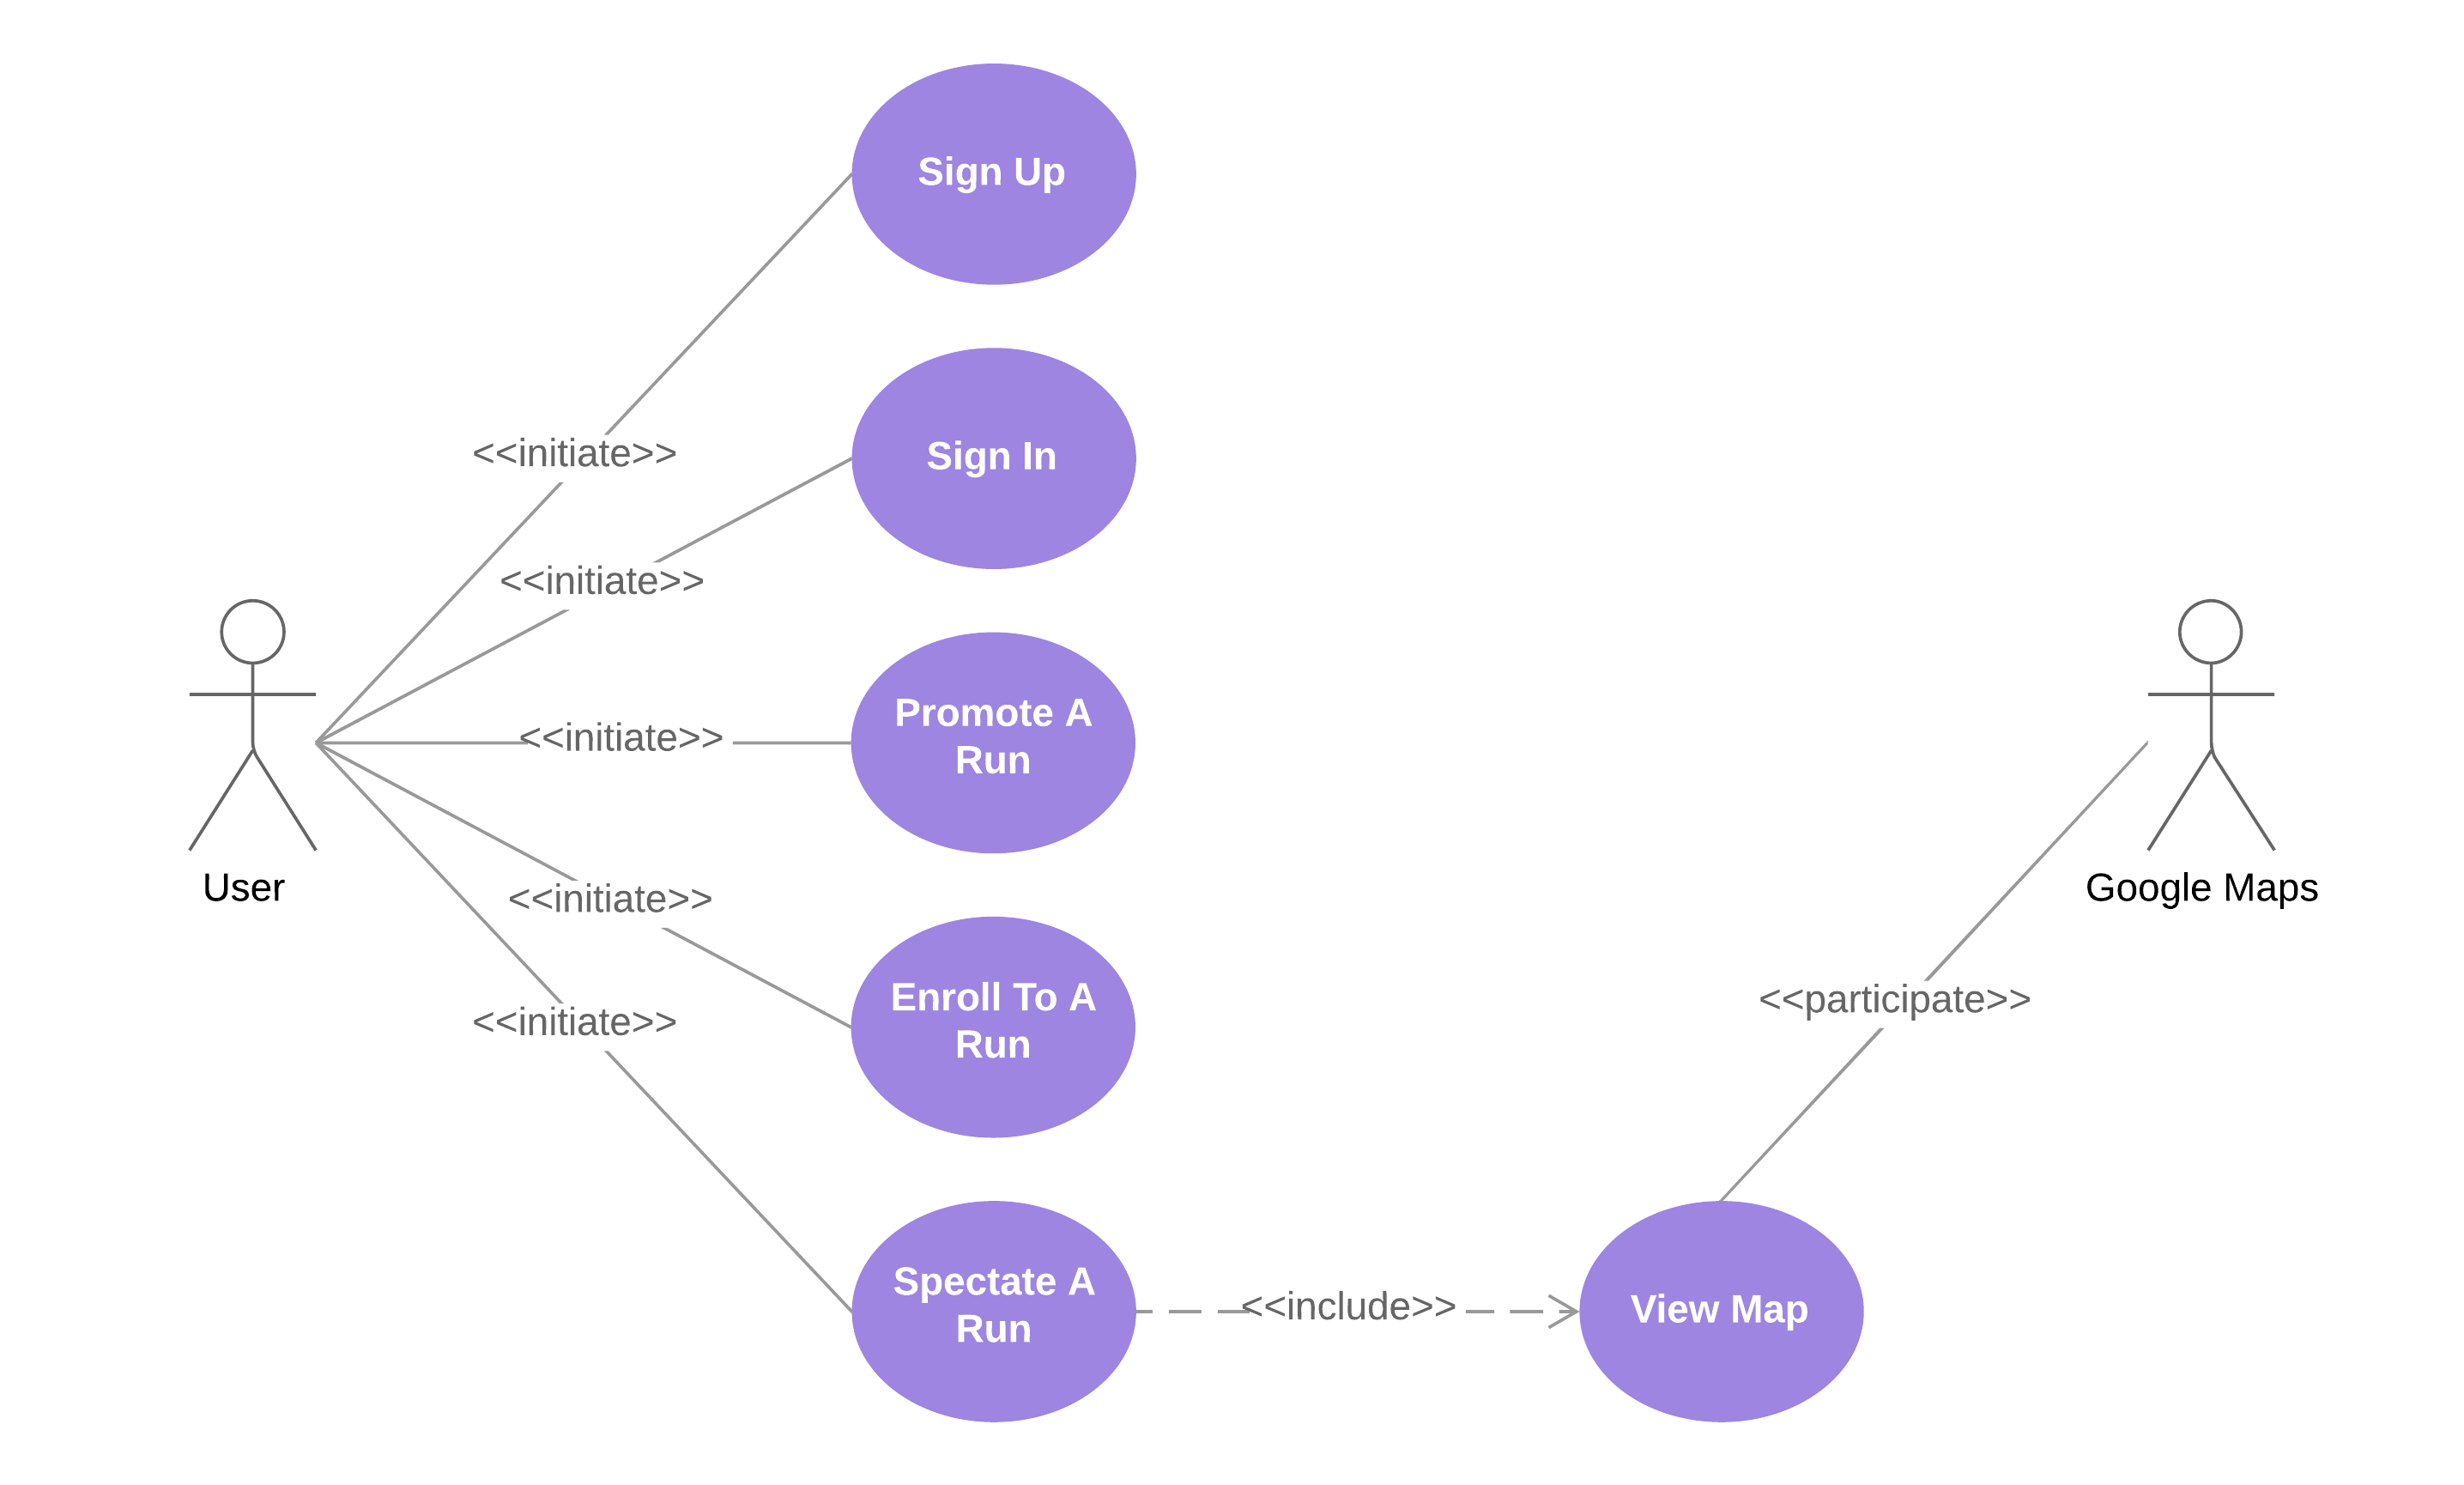
\includegraphics[scale=0.70]{Images/Track4RunCaseDiagram.png}
\end{center}
\FloatBarrier
\end{minipage}
\end{enumerate}

\begin{enumerate}
\FloatBarrier
\item[•]{\Large Data4Help Use Cases}
\FloatBarrier
\begin{table}[h]
\begin{tabular}{|l|p{.75\textwidth}|}
\hline
Name             & Sign Up \\ \hline
Actors           & Third Party \\ \hline
Entry Conditions & The third party has the registration website page opened.    \\ \hline
Event Flow       & \begin{enumerate}
            \item The Third Party clicks on the "Sign Up" button.
            \item The Third Party fills all the attribute fields
            \item The Third Party clicks on "Register Now" button.
            \item The system creates and saves the third party's account.
        \end{enumerate}\\ \hline
Exit Condition   & The third party's account has been created and the third party is now registered.\\ \hline
Exceptions       & \begin{itemize}
\item If the system notices that attributes used in the registration are already linked to an existing account then a warning is generated saying that there is already a third party registered with the given credentials.
\end{itemize}\\ \hline
\end{tabular}
\end{table}
\FloatBarrier

\FloatBarrier
\begin{table}[h]
\begin{tabular}{|l|p{.75\textwidth}|}
\hline
Name             & Sign In \\ \hline
Actors           & Third Party  \\ \hline
Entry Conditions & The third party has the registration website page opened.    \\ \hline
Event Flow       & \begin{enumerate}
            \item The Third Party clicks on the "Sign In" button.
            \item The Third Party fills all credentials fields. 
            \item The Third Party clicks on "Log in" button.
            \item The system accept the log in request.
        \end{enumerate}\\ \hline
Exit Condition   & The third party is now logged in.\\ \hline
Exceptions       & \begin{itemize}
\item If the third party inserts invalid log in credentials a warning is generated saying the credentials are invalid.
\end{itemize}\\ \hline
\end{tabular}
\end{table}
\FloatBarrier

\FloatBarrier
\begin{table}[h]
\begin{tabular}{|l|p{.75\textwidth}|}
\hline
Name             & Request Individual Monitoring \\ \hline
Actors           & Third Party  \\ \hline
Entry Conditions & The third party is logged in.    \\ \hline
Event Flow       & \begin{enumerate}
            \item The Third Party clicks on the "Individual Request" button.
            \item The Third Party inserts the fiscal code or the social security number of the individual to track .
            \item The system shows all the individual's information that have been tracked until the request. 
        \end{enumerate}\\ \hline
Exit Condition   & The request's outcome is shown to the user.\\ \hline
Exceptions       & \begin{itemize}
\item If the inserted fiscal code or social security number are not linked to any account then a warning message is displayed saying that the individual is not registered.
\item If the individual with the fiscal code or social security number inserted didn't accept the individual treatment of data policy then a warning message is displayed saying that the request is rejected.
\end{itemize}\\ \hline
\end{tabular}
\end{table}
\FloatBarrier

\FloatBarrier
\begin{table}[h]
\begin{tabular}{|l|p{.75\textwidth}|}
\hline
Name             & Request Group Monitoring \\ \hline
Actors           & Third Party  \\ \hline
Entry Conditions & The third party is logged in.    \\ \hline
Event Flow       & \begin{enumerate}
            \item The Third Party clicks on the "Group Request" button.
            \item The Third Party inserts the all the attributes that will define the group of interest.
            \item The system accepts the request.
            \item The system shows all the group's information that have been collected until the request. 
        \end{enumerate}\\ \hline
Exit Condition   & The request's outcome is shown.\\ \hline
Exceptions       & \begin{itemize}
\item If the group request get rejected by the system a warning message will be displayed saying the request is rejected.
\end{itemize}\\ \hline
Special Requirements & The system rejects group monitoring requests when the group's information can compromise users' privacy. For this purpose requests of groups composed by less than 1000 users get rejected.
\\ \hline
\end{tabular}
\end{table}
\FloatBarrier

\FloatBarrier
\begin{table}[h]
\begin{tabular}{|l|p{.75\textwidth}|}
\hline
Name             & Subscribe To A Group\\ \hline
Actors           & Third Party  \\ \hline
Entry Conditions & The third party has just sent an accepted monitoring request to a group. \\ \hline
Event Flow       & \begin{enumerate}
            \item Third Party clicks on the "Subscribe to this Group" button.
			\item The system links the third party to the group.            
            \item The system sends new data to the third party.
        \end{enumerate}\\ \hline
Exit Condition   & The Third Party is subscribed to the selected group.\\ \hline
Exceptions       & \begin{enumerate}
            \item If the third party is already subscribed a warning message is shown saying the subscription have been already done.
        \end{enumerate}\\ \hline
\end{tabular}
\end{table}
\FloatBarrier

\FloatBarrier
\begin{table}[h]
\begin{tabular}{|l|p{.75\textwidth}|}
\hline
Name             & Sign Up From Partner App\\ \hline
Actors           & User, Partner Application  \\ \hline
Entry Conditions & The user accepted the treatment of data policy and wants to create an account.  \\ \hline
Event Flow       & \begin{enumerate}
			\item The user start the sign up function on the partner app.
			\item The Partner Application shows to the user all the attributes needed for the registration.
            \item The User fills all the attribute fields.
            \item The Partner Application sends to the system the attributes inserted by the user.
            \item The system receives by the partner application all the attributes inserted by the user.
            \item The system creates the user account and saves the received data.
        \end{enumerate}\\ \hline
Exit Condition   & The system registered the user.\\ \hline
Exceptions       & \begin{itemize}
\item If the system notices that the social security number or fiscal code used in the registration are already linked to an existing account then a message is sent back to the partner application in order to let the user know what happened.
\end{itemize}\\ \hline
\end{tabular}
\end{table}
\FloatBarrier

\FloatBarrier
\begin{table}[h]
\begin{tabular}{|l|p{.75\textwidth}|}
\hline
Name             & Link Account To The Partner App\\ \hline
Actors           & User, Partner Application  \\ \hline
Entry Conditions & The user accepted the treatment of data policy and wants to link his already existing account to the partner application.  \\ \hline
Event Flow       & \begin{enumerate}
			\item The user start the account linking function on the partner app.
			\item The Partner Application shows to the user all the attributes needed for the linking process.
            \item The User fills all the attribute fields.
            \item The Partner Application sends to the system the attributes inserted by the user.
            \item The system receives by the partner application all the attributes inserted by the user.
            \item The system send back to the partner application the outcome of the operation. 
        \end{enumerate}\\ \hline
Exit Condition   & The system registered the user.\\ \hline
Exceptions       & None.\\ \hline
\end{tabular}
\end{table}
\FloatBarrier


\FloatBarrier
\begin{table}[h]
\begin{tabular}{|l|p{.75\textwidth}|}
\hline
Name             & Send User's Data\\ \hline
Actors           & User, Partner Application  \\ \hline
Entry Conditions & The user accepted the treatment of data policy.  \\ \hline
Event Flow       & \begin{enumerate}
            \item The User uses the partner application.
            \item The Partner Application sends the user's information to the the system.
            \item The system receives and saves the user data sent by the partner application.
        \end{enumerate}\\ \hline
Exit Condition   & The system saved the user data.\\ \hline
Exceptions       & None \\ \hline
\end{tabular}
\end{table}
\FloatBarrier

\item[•]{\Large AutomatedSOS Use Cases}
\FloatBarrier
\begin{table}[h]
\begin{tabular}{|l|p{.75\textwidth}|}
\hline
Name             & Sign Up \\ \hline
Actors           & User  \\ \hline
Entry Conditions & The User launched AutomatedSOS on his smartwatch.    \\ \hline
Event Flow       & \begin{enumerate}
            \item The User clicks on the "Sign Up" button.
            \item The User accepts the treatment of data policy.
            \item The User fills all the attribute fields.
            \item The User clicks on "Register Now" button.
            \item The system creates and saves the user's account.
        \end{enumerate}\\ \hline
Exit Condition   & The user's account has been created and the user is now registered.\\ \hline
Exceptions       & \begin{itemize}
\item If the User does not accept the treatment of data policy then a warning is generated saying that ,in order to register, the policy must be accepted.
\item If the system notices that the social security number or fiscal code used in the registration are already linked to an existing account then a warning is generated saying that an account with the given credentials is already registered.
\end{itemize}\\ \hline
\end{tabular}
\end{table}
\FloatBarrier

\FloatBarrier
\begin{table}[h]
\begin{tabular}{|l|p{.75\textwidth}|}
\hline
Name             & Sign In \\ \hline
Actors           & User  \\ \hline
Entry Conditions & The User has AutomatedSOS application installed on his smartwatch.    \\ \hline
Event Flow       & \begin{enumerate}
            \item The User clicks on the "Sign In" button.
            \item The User inserts his social security number or fiscal code and his password.
            \item The User clicks the "Enter" button.
            \item The system accept the log in in request and redirect the user to the menu.
        \end{enumerate}\\ \hline
Exit Condition   & The User user is now logged in.\\ \hline
Exceptions       & \begin{itemize}
\item If user inserts invalid log in credentials a warning is generated saying the credentials are invalid.
\end{itemize}\\ \hline
\end{tabular}
\end{table}
\FloatBarrier

\FloatBarrier
\begin{table}[h]
\begin{tabular}{|l|p{.75\textwidth}|}
\hline
Name             & See Acquired Data \\ \hline
Actors           & User  \\ \hline
Entry Conditions & The User is logged in. \\ \hline
Event Flow       & \begin{enumerate}
            \item The User clicks on the "Acquired Info" button.
            \item The system gets all the user information that have been retrieved by the application until that moment.
            \item The system display the user information.
\end{enumerate}\\ \hline
Exit Condition   & All the information retrieved by the system are shown on the app.\\ \hline
Exceptions       & \begin{itemize}
\item If the system do not find information about the user then a warning message is shown to the user saying that until now the application did not record any information.
\end{itemize}  \\ \hline
\end{tabular}
\end{table}
\FloatBarrier

\FloatBarrier
\begin{table}[h]
\begin{tabular}{|l|p{.75\textwidth}|}
\hline
Name             & Monitor Current Health \\ \hline
Actors           & User  \\ \hline
Entry Conditions & The User is logged in. \\ \hline
Event Flow       & \begin{enumerate}
            \item The User clicks the "Monitor Health" button.
            \item The system shows in real time all the health values that are being retrieved.
        \end{enumerate}\\ \hline
Exit Condition   & All the health parameters retrieved by the application are shown in real time on the app.\\ \hline
Exceptions       & \begin{itemize}
\item If no health parameters are retrieved a warning message is displayed saying to the user he actually must wear the smartwatch in order to see parameters in real time. 
\end{itemize} \\ \hline
\end{tabular}
\end{table}
\FloatBarrier

\FloatBarrier
\begin{table}[h]
\begin{tabular}{|l|p{.75\textwidth}|}
\hline
Name             & Send Ambulance Request \\ \hline
Actors           & AutomatedSOS, First Aid  \\ \hline
Entry Conditions & A critical health parameter value is below the threshold.
\\ \hline
Event Flow       & \begin{enumerate}
            \item AutomatedSOS sends to First Aid a form that contains all important information about the user, like his current location, his gender, his age, his health profile, and the list of parameters that got below the threshold.
            \item First Aid sends an acknowledge message to AutomatedSOS 
            \item First Aid sends immediately an ambulance to the user's location.
            \item AutomatedSOS displays on the app a warning message saying that an ambulance is currently heading to the user's location. 
        \end{enumerate}
\\ \hline
Exit Condition   & A warning message is shown saying that an ambulance is currently heading to the user's location.
\\ \hline
Exceptions       & \begin{itemize}
\item If no acknowledge message is received by AutomatedSOS after the form has been sent, as soon as a certain time out expires AutomatedSOS re-send the form with updated information. 
\end{itemize}
\\ \hline
Special Requirements & The form need to be sent to First Aid with a reaction time of less than 5 seconds from the time the parameters are below the threshold.
\\ \hline 
\end{tabular}
\end{table}
\FloatBarrier

\FloatBarrier
\item[•]{\Large Track4Run Use Cases}
\begin{table}[h]
\begin{tabular}{|l|p{.75\textwidth}|}
\hline
Name             & Sign Up \\ \hline
Actors           & User  \\ \hline
Entry Conditions & The User has Track4Run application installed on his device.    \\ \hline
Event Flow       & \begin{enumerate}
            \item The User clicks on the "Sign Up" button.
            \item The User accepts the treatment of data policy.
            \item The User fills all the attribute fields.
            \item The User clicks on the "Register Now" button.
            \item The system creates and saves the user's account.
        \end{enumerate}\\ \hline
Exit Condition   & The user's account has been created and the user is now registered.\\ \hline
Exceptions       & \begin{itemize}
\item If the User does not accept the treatment of data policy then a warning is generated saying that ,in order to register, the policy must be accepted.
\item If the system notices that the social security number or fiscal code used in the registration are already linked to an existing account then a warning is generated saying that an account with the given credentials is already registered.
\end{itemize}\\ \hline
\end{tabular}
\end{table}
\FloatBarrier

\FloatBarrier
\begin{table}[h]
\begin{tabular}{|l|p{.75\textwidth}|}
\hline
Name             & Sign In \\ \hline
Actors           & User  \\ \hline
Entry Conditions & The User has Track4Run application installed on his smartwatch.    \\ \hline
Event Flow       & \begin{enumerate}
            \item The User clicks on the "Sign In" button.
            \item The User inserts his social security number or fiscal code and his password.
            \item The User clicks the "Enter" button.
            \item The system accept the log in in request and redirect the user to the menu.
        \end{enumerate}\\ \hline
Exit Condition   & The User user is now logged in.\\ \hline
Exceptions       & \begin{itemize}
\item If user inserts invalid log in credentials a warning is generated saying the credentials are invalid.
\end{itemize}\\ \hline
\end{tabular}
\end{table}
\FloatBarrier

\FloatBarrier
\begin{table}[h]
\begin{tabular}{|l|p{.75\textwidth}|}
\hline
Name             & Promote A Run \\ \hline
Actors           & User  \\ \hline
Entry Conditions & The User is logged in.    \\ \hline
Event Flow       & \begin{enumerate}
            \item The User clicks on the "Promote a Run" button.
            \item The system show a new tab where the user can define the path, name, date and athletes.
            \item The system create the event and adds it to the event list visible in the "Enroll to A Run" section.
            \item The system automatically sends notifications to all athletes specified by the promoter asking them if they want to participate to the run.
        \end{enumerate}\\ \hline
Exit Condition   & The run event has been created and is visible in the list of promoted events.\\ \hline
Exceptions       & \begin{itemize}
\item If the user do not insert critical information (like the path, the name or the date) a warning message is shown saying that critical parameters are missing. The user can close the warning message and fill the remaining parameters or cancel the operation, going back to the main menu.
\end{itemize}\\ \hline
\end{tabular}
\end{table}
\FloatBarrier

\FloatBarrier
\begin{table}[h]
\begin{tabular}{|l|p{.75\textwidth}|}
\hline
Name             & Enroll To A Run \\ \hline
Actors           & User  \\ \hline
Entry Conditions & The User is logged in.    \\ \hline
Event Flow       & \begin{enumerate}
            \item The User clicks on the "Enroll to a Run" button.
            \item The system shows a new tab where the list of all runs created is visible.
            \item The User can filter the runs with attributes like the name, the date and the location.
            \item The User clicks on the specific run he wants to participate to.
            \item The system adds the user to the list of athletes enrolled to the run.
        \end{enumerate}\\ \hline
Exit Condition   & The user is inside the list of athletes of the run.\\ \hline
Exceptions       & \begin{itemize}
\item If the number of athletes has already capped the max amount in the run clicked by the user then a warning message is displayed saying that no more athletes are allowed to participate to the run.
\item If the user didn't accept the treatment of data policy, a warning message is displayed, asking the user to accept it in order to enroll to the run.
\end{itemize}\\ \hline
\end{tabular}
\end{table}
\FloatBarrier

\FloatBarrier
\begin{table}[h]
\begin{tabular}{|l|p{.75\textwidth}|}
\hline
Name             & Spectate A Run \\ \hline
Actors           & User  \\ \hline
Entry Conditions & The User is logged in.    \\ \hline
Event Flow       & \begin{enumerate}
            \item The User clicks on the "Spectate a Run" button.
            \item The system shows a new tab where the list of all live runs is visible.
            \item The User can filter the runs with attributes like the name, and the location.
            \item The User clicks on the specific run he wants to spectate.
            \item The system opens a tab which contains the map of the run and also the position of all athletes in real time.
        \end{enumerate}\\ \hline
Exit Condition   & The spectator tab on the application is open.\\ \hline
Exceptions       & None.\\ \hline
\end{tabular}
\end{table}
\FloatBarrier

\FloatBarrier
\begin{table}[h]
\begin{tabular}{|l|p{.75\textwidth}|}
\hline
Name             & View Map \\ \hline
Actors           & AutomatedSOS  \\ \hline
Entry Conditions & The user has just started spectating a run. \\ \hline
Event Flow       & \begin{enumerate}
            \item AutomatedSOS uses Google Maps API in order to retrieve the map of the run.
            \item AutomatedSOS represents athletes on the map in their current position.
        \end{enumerate}\\ \hline
Exit Condition   & The current position of athletes is present on the map of the run.\\ \hline
Exceptions       & None.\\ \hline
\end{tabular}
\end{table}
\FloatBarrier

\end{enumerate}


\subsection{Sequence Diagram}
\begin{enumerate}
\begin{minipage}{\textwidth}
\FloatBarrier
\item[•]{\Large Data4Help}


Individual request with on-demand acquisition performance.
\begin{center}
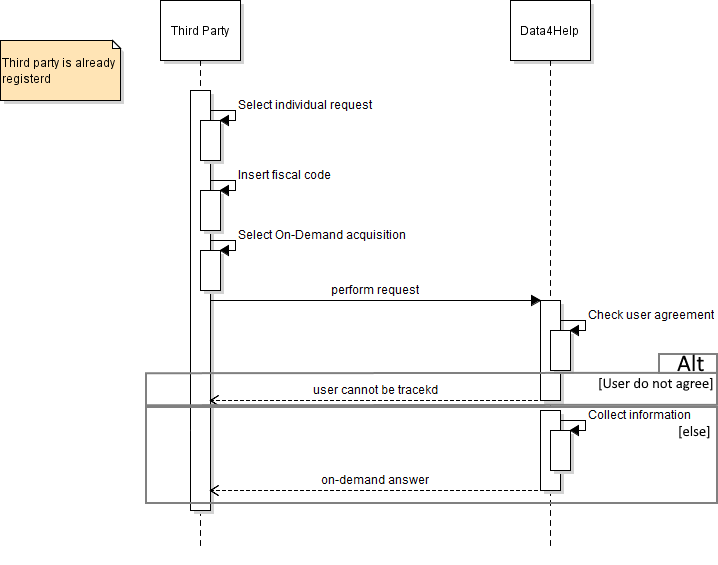
\includegraphics[scale=0.8]{Images/Seq_Data4Help_onDem.png}
\end{center}
\FloatBarrier

\FloatBarrier
Automatic data update inside Data4Help:
\begin{center}
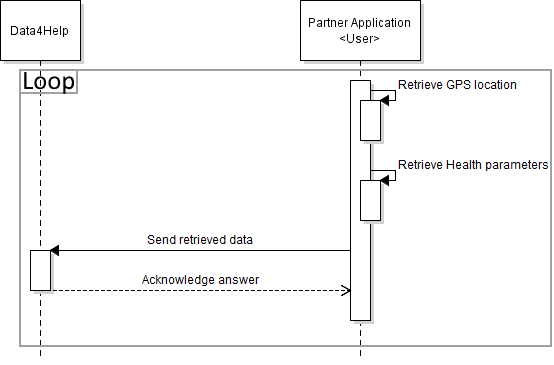
\includegraphics[scale=0.8]{Images/Seq_Data4Help_autoUp.png}
\end{center}
\FloatBarrier

\end{minipage}

\begin{minipage}{\textwidth}
\FloatBarrier
Group request with live acqusition performance:
\begin{center}
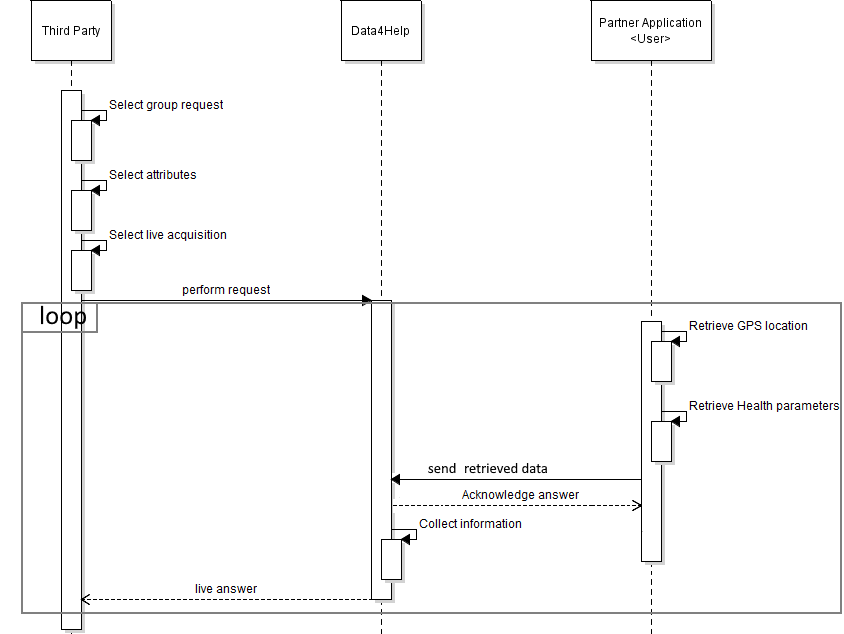
\includegraphics[scale=0.75]{Images/Seq_Data4Help_live.png}
\end{center}

\FloatBarrier
User registration performance:
\begin{center}
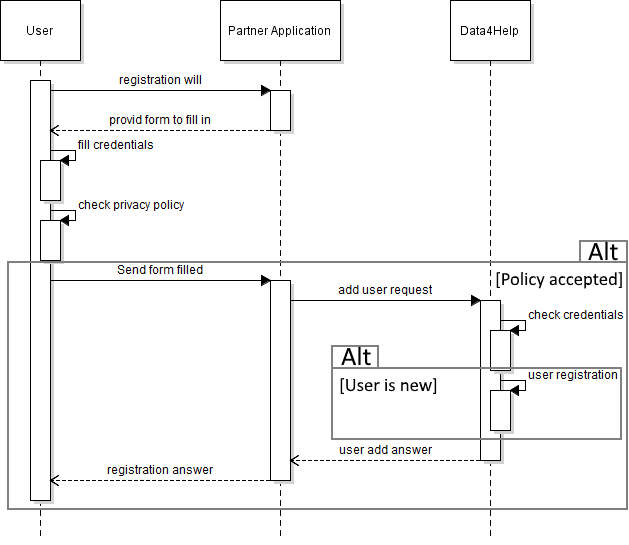
\includegraphics[scale=0.75]{Images/Seq_Data4Help_registration.png}
\end{center}


\FloatBarrier
\end{minipage}


\begin{minipage}{\textwidth}
\item[•]{\Large AutomatedSOS}
\FloatBarrier
AutomatedSOS monitor and ambulance caller services:
\begin{center}
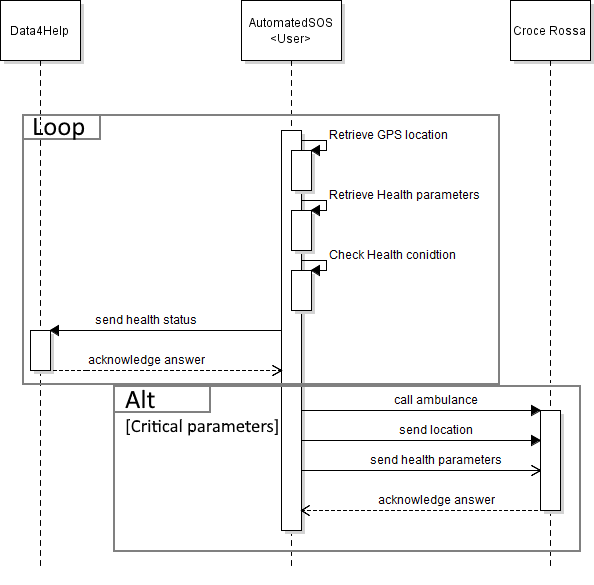
\includegraphics[scale=0.8]{Images/Seq_AutoSOS_monitor.png}
\end{center}
\FloatBarrier

\item[•]{\Large Track4Run}
\FloatBarrier
Track4Run automated retrieve athletes' position and update spectators' live map.
\begin{center}
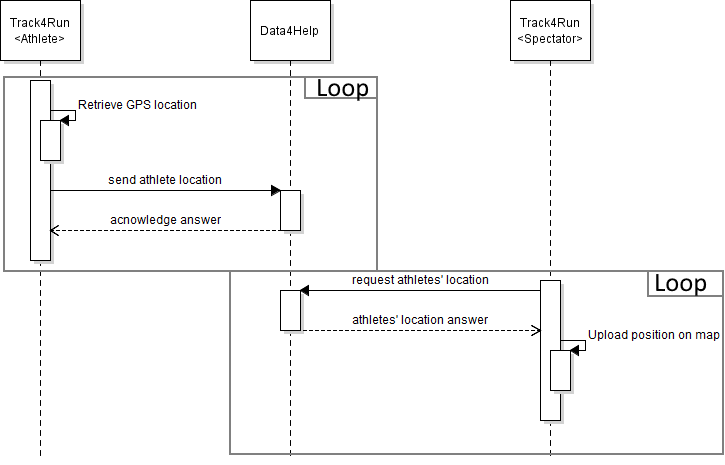
\includegraphics[scale=0.8]{Images/Seq_Track4Run_raceUp.png}
\end{center}
\FloatBarrier
\end{minipage}

\end{enumerate}


\subsection{Performance Requirements}
\begin{enumerate} 
\item[•] Data4Help service is build to perform trend research from users that download specific partner applications, in order to perform this type of monitoring there is a high use of resources (specially in live acquisition when data must be exchanged within 2 minutes) therefore ,initially, this application is developed to track 10.000 users simultaneously (included users from AutomateSOS and Track4Run). To serve third parties is required less performance because they are very few in comparison to users.

\item[•] AutomatedSOS is a very expensive application in terms of performance because it must monitor the individual all the day and guarantee a data collection with an interval of 2 seconds.

\item[•] Track4Run is a variable expensive application because it has to monitor individual constantly during the race, but not all day, all the athletes have a run.
\end{enumerate}

\subsection{Design Constraints}
\subsubsection{Standards compliance}
\begin{enumerate} 
\item[•] Partner applications request the permission to retrieve location and health status to the device, same for AutomateSOS and Track4Run.
\item[•] Data4Help requires that partner applications can use internet connection and users' mobile data to exchange information.
\item[•] AutomatedSOS requires all day internet connection in order to call an ambulance every time is needed.
\item[•] AutomatedSOS requires internet connection during all the duration of the race to the athletes and to the spectator.
\end{enumerate}

\subsubsection{Hardware limitations}
\begin{enumerate} 
\item[•] AutomatedSOS application requires that is installed on a smartwatch (smartphone is not enough) in order to acquire location and health status.
\item[•] Track4Run application requires that is installed on a smartphone (or a smartwatch) in order to acquire location.
\item[•] Smartphone and smartwatch must be iOS or Android platform.
\item[•] The devices must have internet connection (mobile data are mandatory).
\item[•] The devices must have GPS locator.
\item[•] Smartwatch must have Heart Rate monitor, Blood Pressure monitor, Pedometer, Calories Calculator.
\end{enumerate}

\subsection{Software System Attributes}
\subsubsection{Reliability}
\subsubsection{Availability}
\subsubsection{Security}
\subsubsection{Maintainability}
\subsubsection{Portability}
